%%%%%%%%%%%%%%%%%%%%%%%%%%%%%%%%%%%%%%%%%%%%%%%%%%%%%%%%%%%%%%%%%%%%%%%%
\chapter{Elementi di teoria degli {\em ensembles}}
\label{cap:elementi}
%%%%%%%%%%%%%%%%%%%%%%%%%%%%%%%%%%%%%%%%%%%%%%%%%%%%%%%%%%%%%%%%%%%%%%%%

%%%%%%%%%%%%%%%%%%%%%%%%%%%%%%%%%%%%%%%%%%%%%%%%%%%%%%%%%%%%%%%%%%%%%%%%
\section{Introduzione}
%%%%%%%%%%%%%%%%%%%%%%%%%%%%%%%%%%%%%%%%%%%%%%%%%%%%%%%%%%%%%%%%%%%%%%%%

Consideriamo un sistema fisico macroscopico all'equilibrio termico e meccanico: ciò ci rassicura sulla persistenza, col passare del tempo, dello stesso macrostato di partenza. Se però potessimo guardare il sistema da un punto di vista microscopico ci accorgeremmo senza dubbio che il sistema stesso passa in continuazione da un microstato all'altro. Potremmo dire che il sistema {\em esplora} senza sosta tutti i microstati compatibili col macrostato d'equilibrio.

Se ora effettuiamo una misura di un qualsiasi osservabile fisico $f$ (per esempio la pressione esercitata sulle pareti del contenitore) abbiamo a disposizione (almeno) due punti di vista teorici per interpretare il dato ricavato: dal lato macroscopico possiamo dirci che posta la situazione d'equilibrio il valore di $f$ non cambia (a parte le inevitabili fluttuazioni, sulle quali necessariamente mediamo) se siamo abbastanza accorti da non perturbare il sistema durante la misura\footnote{Cioè se siamo abbastanza accorti da perturbarlo in maniera a tutti gli effetti pratici ininfluente.}, e quindi possiamo prenderci tutto il tempo del mondo. Da un punto di vista microscopico, durante l'atto di misura (che durerà necessariamente un tempo macroscopicamente finito) il sistema passerà attraverso moltissimi microstati compatibili col macrostato osservato: abbiamo dunque tutti i diritti di ritenere che la nostra misura sarà in realtà il risultato di una {\em media dell'osservabile su tutti i microstati esplorati dal sistema}.

Nulla ci vieta di considerare le cose sotto un ottica più astratta: al tempo fissato $t$ replichiamo mentalmente il sistema, ottenendone $\calN$ copie immaginarie tutte nello stesso stato macroscopico ma distribuite tra tutti i microstati possibili. Una qualsiasi di queste $\calN$ {\em copie mentali} (il cui insieme è conosciuto col nome di {\em ensemble statistico}) è una possibile rappresentante del sistema, e sembra naturale concludere che l'operazione di media temporale {\em sul singolo sistema fisico originale} sia sostanzialmente equivalente (sotto certe ipotesi che vaglieremo in seguito) all'operazione di media {\em sugli elementi dell'ensemble}. Quest'idea è il nucleo centrale della teoria degli \ensembles.

%%%%%%%%%%%%%%%%%%%%%%%%%%%%%%%%%%%%%%%%%%%%%%%%%%%%%%%%%%%%%%%%%%%%%%%%
\section{Spazio delle fasi di un sistema classico}
%%%%%%%%%%%%%%%%%%%%%%%%%%%%%%%%%%%%%%%%%%%%%%%%%%%%%%%%%%%%%%%%%%%%%%%%

Se consideriamo le cose da un punto di vista classico, definire un microstato del sistema (stiamo pensando a un sistema macroscopico costituito da $N$ particelle considerate come elementari) significa assegnare, a un tempo fissato $t_{0}$, posizione e velocità (momento) a ogni particella; se conosciamo tutte le forze che agiscono sulle particelle, le equazioni del moto saranno poi sufficienti a ricavare il microstato in ogni istante di tempo posteriore a $t_{0}$.

Assegnare tutte le posizioni e tutti i momenti corrisponde a definire un vettore (reale) con $6N$ componenti:
\be
\myvec{r} = (q_{1}, q_{2}, q_{3}, \dots q_{3N}, p_{1}, p_{2}, p_{3}, \dots p_{3N})
\ee
e il vettore $\myvec{r}$ definisce un punto (detto {\em punto rappresentativo} del sistema) in uno spazio a $6N$ dimensioni: il famigerato {\em spazio delle fasi}. Le componenti $(q_{i},p_{i})$ dipendono naturalmente dal tempo, e il modo in cui variano è dettato dalle equazioni del moto di Hamilton:
\bea
\label{eq:eqmotoH}
\dot{q}_{i} &=&   \dpar{\Ham(q_{i}, p_{i})}{p_{i}}\nonumber\\
\dot{p}_{i} &=& - \dpar{\Ham(q_{i}, p_{i})}{q_{i}}
\eea
in cui $\Ham$ è ovviamente la funzione Hamiltoniana del sistema. Il punto rappresentativo descriverà dunque, al passare del tempo, una certa traiettoria nello spazio delle fasi $\Phi$, traiettoria che di necessità rimarrà confinata in una regione {\em finita} di $\Phi$: questo perché la {\em scatola} che racchiude il sistema limita i possibili valori delle $q_{i}$, mentre il valore finito dell'energia $E$ limita i possibili valori delle $p_{i}$.

Se l'energia ha un valore fissato e preciso, $E$, la traiettoria rimarrà confinata su un'ipersuperficie di $\Phi$ definita dall'equazione
\be
\Ham(q_{i}, p_{i}) = E
\ee
Consideriamo ora un \ensemble: ogni elemento, a ogni istante di tempo $t$, sarà rappresentato da un punto in $\Phi$: otteniamo quindi l'immagine di uno {\em sciame} di punti rappresentativi che, confinati nella giusta regione di $\Phi$, si spostano in accordo con le leggi del moto.

Introduciamo una funzione densità $\rho(q,p;t)$. Consideriamo un punto $(q,p)$ nello spazio delle fasi, un volumetto infinitesimale
\be
\dephi \equiv \mbox{d}^{3N}q\;\mbox{d}^{3N}p
\ee
intorno a esso, e un \ensemble\ che descriva un certo macrostato del sistema. 
Sia $\de{\calN}(q,p;t)$ il numero di punti rappresentativi dell'\ensemble\ contenuti in $\dephi$ al tempo $t$.
Possiamo definire la funzione densità $\rho(q,p;t)$:
\be
\rho(q,p;t)\dephi = \lim_{\calN\to\infty}\dfrac{\de{\calN}(q,p;t)}{\calN}
\ee
La densità $\rho$ rappresenta quindi il modo in cui sono distribuiti i punti rappresentativi nello spazio delle fasi, ed è definita come una densità di probabilità, perché è semidefinita positiva e inoltre, ovviamente, a ogni tempo $t$ abbiamo
\be
\label{eq:normarho}
\int\dephi\rho(q,p;t) = 1
\ee
Per definizione di media sull'\ensemble\ possiamo scrivere, per un generico osservabile fisico $f$:
\be
\aspetta{f} = \int\dephi \rho(q,p;t) f(q,p)
\ee
ricordando che, vedi la (\ref{eq:normarho}), la densità è normalizzata.
Nella definizione di media l'integrale è preso sull'intero spazio delle fasi, ma chiaramente solo le regioni in cui $\rho(q,p;t)$ è diversa da zero daranno contributo. Notiamo che attraverso la dipendenza esplicita dal tempo di $\rho$ anche $\aspetta{f}$ può, in linea di principio, dipendere dal tempo. Ci occuperemo ora proprio della possibile dipendenza di $\rho$ dal tempo e di come questa può influire sul sistema fisico in esame, senza dimenticare che siamo interessati a sistemi fisici all'equilibrio, i cui parametri macroscopici quindi non dipendono dal tempo. In particolare non dobbiamo dimenticare che anche scegliendo una densità che non dipenda {\em esplicitamente} dal tempo, $\rho$ potrebbe ancora dipendere {\em implicitamente} dal tempo tramite la dipendenza da $(q,p)$.

%%%%%%%%%%%%%%%%%%%%%%%%%%%%%%%%%%%%%%%%%%%%%%%%%%%%%%%%%%%%%%%%%%%%%%%%
\subsection{Il teorema di Liouville}
%%%%%%%%%%%%%%%%%%%%%%%%%%%%%%%%%%%%%%%%%%%%%%%%%%%%%%%%%%%%%%%%%%%%%%%%

%%%%%%%%%%%%%%%%%%%%%%%%%%%%%%%%%%%%%%%%%%%%%%%%%%%%%%%%%%%
%\begin{figure}[!ht]
%  \centering
%  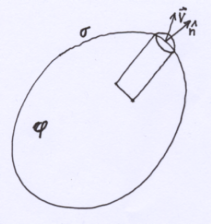
\includegraphics[width=0.6\textwidth]{liouville.png}
%  \caption{Il teorema di Liouville}
%  \label{fig:liouville}
%\end{figure}
%%%%%%%%%%%%%%%%%%%%%%%%%%%%%%%%%%%%%%%%%%%%%%%%%%%%%%%%%%%

Il teorema di Lioville stabilisce che la densità $\rho(q,p;t)$ si comporta come un {\em fluido incomprimibile}. Per vederlo, consideriamo l'evoluzione nel tempo di $\de{\calN}$. Prendiamo un punto rappresentativo $(q,p)$ all'interno del volumetto $\dephi$ al tempo $t$. Dopo in intervallo di tempo $\delta t$ il punto $(q,p)$ si sarà spostato in $(q',p')$, con
\bea
\label{eq:spostaqp}
q_i' &=& q_i + \dot{q}_i\delta t + O(\delta t^2) \nonumber \\
p_i' &=& p_i + \dot{p}_i\delta t + O(\delta t^2)
\eea
L'elemento di volume originale, $\dephi$, è un ipercubo. Dopo lo spostamento risulterà distorto, e dobbiamo calcolare il nuovo elemento di volume $\dephi' = \prod_i \de{q_i'}\de{p_i'}$. Possiamo subito scrivere
\bea
\de{q_i'} &=& \de{q_i} + \dpar{\dot{q}_i}{q_i}\de{q_i} \delta t+O(\delta t^2) \nonumber \\
\de{p_i'} &=& \de{p_i} + \dpar{\dot{p}_i}{p_i}\de{p_i} \delta t+O(\delta t^2) \nonumber
\eea
Dalla precedente segue che per ciascuna coppia coniugata abbiamo
\be
\label{eq:evolvol}
\de{q_i'}\de{p_i'} = \de{q_i}\de{p_i}\left[
1 + \left(
\dpar{\dot{q}_i}{q_i} + \dpar{\dot{p}_i}{p_i}
\right)\delta t + O(\delta t^2)
\right]
\ee
Le equazioni del moto (\ref{eq:eqmotoH}) ci dicono però che
\be
\dpar{\dot{q}_i}{q_i} = \dfrac{\partial}{\partial q_i}\dpar{\Ham}{p_i}
= \dfrac{\partial^2\Ham}{\partial q_i\partial p_i}
\ee
e che
\be
\dpar{\dot{p}_i}{p_i} = -\dfrac{\partial}{\partial p_i}\dpar{\Ham}{q_i}
= -\dfrac{\partial^2\Ham}{\partial q_i\partial p_i}
\ee
Il termine proporzionale a $\delta t$ nella (\ref{eq:evolvol}) si annulla dunque per le equazioni del moto, e otteniamo $\dephi' = \dephi$. Questo significa che tutti i punti rappresentativi $\de{\calN}$ originariamente vicini al punto $(q,p)$ vengono trasportati nelle immediate vicinanze di $(q',p')$ in modo tale da preservare il volume occupato. Il rapporto $\de{\calN}/\dephi$ rimane invariato, che è un altro modo di dire che $\rho$ si comporta come  un fluido incomprimibile.

Introducendo le parentesi di Poisson
\be
\label{eq:parentesi-poisson}
\{\rho,\Ham\} = \sum_{i}\left( \dpar{\rho}{q_{i}}\dpar{\Ham}{p_{i}} - \dpar{\rho}{p_{i}}\dpar{\Ham}{q_{i}} \right)
\ee
la condizione di incomprimibilità, $\rho(q',p';t+\de{t}) = \rho(q,p;t)$ può finalmente essere scritta, in forma differenziale, in questo modo:
\be
\label{eq:liouville}
\dfrac{\de{\rho}}{\de{t}} = \dpar{\rho}{t} + \{\rho,\Ham\} = 0
\ee
che è appunto il {\em teorema di Liouville}. 

Ricordiamo ora che siamo interessati alla descrizione di sistemi macroscopici all'equilibrio; il valore d'aspettazione di qualsiasi osservabile deve essere costante nel tempo, o meglio, indipendente dal tempo. In questo caso abbiamo che $\rho$ stessa non può dipendere esplicitamente dal tempo; dobbiamo certamente imporre, come primo passo, la condizione di stazionarietà:
\be
\dpar{\rho}{t} = 0
\ee
A questo punto siamo costretti anche a chiedere che le parentesi di Poisson si annullino:
\be
\label{eq:parpois0}
\{\rho,\Ham\} = 0
\ee
Si vede subito che $\rho$ non può essere un'arbitraria funzione di $(q,p)$, ma dev'essere una funzione dell'hamiltoniana del sistema. Il modo più semplice di implementare la condizione (\ref{eq:parpois0}) è quella di assumere $\rho$ costante sulla ipersuperficie a energia costante $E$ nello spazio delle fasi. Ciò corrisponde a considerare l'\ensemble\ micronanonico.

%%%%%%%%%%%%%%%%%%%%%%%%%%%%%%%%%%%%%%%%%%%%%%%%%%%%%%%%%%%%%%%%%%%%%%%%
\section{L'\ensemble\ microcanonico}
%%%%%%%%%%%%%%%%%%%%%%%%%%%%%%%%%%%%%%%%%%%%%%%%%%%%%%%%%%%%%%%%%%%%%%%%

Consideriamo dunque un sistema fisico in cui le grandezze macroscopiche fondamentali siano il numero di particelle, $N$, il volume $V$ in cui sono racchiuse e l'energia totale $E$ del sistema stesso, che si suppone conservata (sistema isolato). La terna $(N,\,V,\,E)$ rappresenta quindi un macrostato del sistema.

In realtà pensare di tenere l'energia esattamente fissata non è una buona idea; per modellizzare meglio una situazione fisica reale possiamo pensare a un sistema in cui l'energia possa variare di una quantità $\pm \Delta/2$ intorno al valore centrale $E$ (con la condizione naturalmente che $\Delta \ll E$).

La condizione
\be
\Ham(q,p) = E
\ee
definisce una ipersuperficie ($6N-1$ dimensionale) nello spazio delle fasi $\Phi$. Sia ora $\gamma$ il volume nello spazio delle fasi definito dalla condizione
\be
E-\frac{\Delta}{2} \le \Ham \le E+\frac{\Delta}{2}
\ee
ossia il volume del guscio di spessore $\Delta$ intorno alla ipersuperficie a energia costante $E$. L'ensemble microcanonico è definito dalla condizione che $\rho$ sia costante all'interno del volume $\gamma$ e sia nulla all'esterno. Abbiamo dunque
\be
\gamma = \int\limits_{E-\frac{\Delta}{2} \le \Ham \le E+\frac{\Delta}{2}}\dephi
\ee

Con queste definizioni otteniamo, per il valore d'aspettazione di una generica osservabile, l'equazione
\be
\aspetta{A} = \frac{1}{\gamma}\int\limits_\gamma A(q,p)\dephi
\ee

Prima di considerare il numero di microstati $\Gamma$ e il suo rapporto con $\gamma$, è giunto il momento di svelare una drammatica verità: la meccanica statistica classica non è ben fondata. Ciò dovrebbe essere intuitivo: la meccanica statistica ha a che fare col comportamento dei costituenti microscopici di un sistema macroscopico, e nel mondo microscopico valgono le regole quantistiche. Un corretto conto dei microstati può essere effettuato solo col formalismo quantistico. Dunque da un punto di vista logico sarebbe più giusto fondare la meccanica statistica sul formalismo quantistico e poi vedere sotto quali condizioni si può ricavare la meccanica statistica classica. Questo però non è stato il percorso storico, e dal punto di vista didattico è preferibile seguire la stessa strada dei padri fondatori della meccanica statistica.

Dovrebbe essere chiaro che il valore del volume $\gamma$ ha qualcosa a che fare $\Gamma$ ma in ogni caso $\gamma$ non coincide con il numero dei microstati. Per stabilire una corrispondenza numerica precisa occorre trovare un ``volume fondamentale'' $\gamma_{0}$, il cui significato fisico è il seguente: a un microstato del sistema corrisponde un volume $\gamma_{0}$ nello spazio delle fasi. Avremo dunque
\be
\Gamma = \gamma/\gamma_{0}
\ee
e quindi
\be
S = k \ln(\gamma/\gamma_{0})
\ee
Tutto ciò dovrebbe essere intuitivo: infatti da un punto di vista quantistico l'idea di {\em punto rappresentativo} nello spazio delle fasi perde senso, perché a causa delle relazioni di indeterminazione di Heisemberg non possiamo specificare con precisione arbitraria sia la posizione $q$ sia il momento $p$ di una particella. Il meglio che possiamo fare è quello di assumere che il punto divenga, appunto, un volumetto $\gamma_0$.

Il problema è dunque quello di trovare $\gamma_{0}$. Lo faremo servendoci di un ``trucco'': considereremo un paio di sistemi semplici e calcoleremo $\gamma$ nel caso classico (nel quale il volume nello spazio delle fasi ha significato) e $\Gamma$ col formalismo quantistico. Il rapporto tra i due risultati darà il valore di $\gamma_{0}$.

%%%%%%%%%%%%%%%%%%%%%%%%%%%%%%%%%%%%%%%%%%%%%%%%%%%%%%%%%%%%%%%%%%%%%%%%
\subsection{Il gas ideale}
%%%%%%%%%%%%%%%%%%%%%%%%%%%%%%%%%%%%%%%%%%%%%%%%%%%%%%%%%%%%%%%%%%%%%%%%

Abbiamo come al solito $N$ particelle identiche non interagenti racchiuse in un volume $V$. L'hamiltoniana del sistema è 
\be
\Ham = \sum_{i=1}^{3N}\frac{p^2_i}{2m}
\ee
in cui $m$ è la massa delle particelle. Abbiamo
\be
\gamma = \int\limits_{E-\frac{\Delta}{2} \le \Ham \le E+\frac{\Delta}{2}}\dephi
\ee
L'integrazione sulle coordinate dà semplicemente un fattore $V^{N}$ perché l'Hamiltoniana non dipende dalle coordinate ma solo dai momenti. Abbiamo dunque
\be
\gamma = V^N\int\limits_{2m(E-\Delta/2)\le\sum_i p_{i}^{2}\le 2m(E+\Delta/2)}\de^{3N} p
\ee
$\gamma$ rappresenta il volume di un iperguscio confinato tra due ipersfere di raggi rispettivamente $\sqrt{2m(E-\Delta/2)}$ (raggio interno) e $\sqrt{2m(E+\Delta/2)}$ (raggio esterno). Per $\Delta \ll E$ possiamo scrivere $\sqrt{2m(E\pm\Delta/2)}\simeq\sqrt{2mE}(1\pm\Delta/4E)$ e lo spessore del guscio risulta quindi pari a $R_{+}-R_{-}\simeq\Delta\sqrt{m/2E}$. Moltiplicando questo valore per la superficie dell'ipersfera di raggio $\sqrt{2mE}$ otteniamo con buona approssimazione il volume del guscio. Utilizzando il risultato per la superficie di un'ipersfera in $n$ dimensioni, ossia
\be
S_{n}(R) = \frac{2\pi^{n/2}}{\Gamma(n/2)}R^{n-1}
\ee
otteniamo, considerando che $n = 3N$:
\be
\gamma \simeq \frac{\Delta}{E}V^{N}\frac{(2\pi mE)^{3N/2}}{(3N/2 - 1)!}
\ee
Nel caso quantistico avevamo ottenuto (vedi capitolo precedente)
\be
\Gamma \simeq \frac{\Delta}{E}\frac{V^{N}}{h^{3N}}\frac{(2\pi mE)^{3N/2}}{(3N/2 - 1)!}
\ee
e dal confronto otteniamo subito
\be
\gamma_{0}\equiv(\gamma/\Gamma) = h^{3N}
\ee
Notiamo che dal punto di vista dimensionale le cose tornano: il prodotto di una posizione $q$ per un momento $p$ dà un oggetto che ha le dimensioni di un momento angolare, e $\gamma_0$ deve proprio avere le dimensioni di un momento angolare alla $3N$

%%%%%%%%%%%%%%%%%%%%%%%%%%%%%%%%%%%%%%%%%%%%%%%%%%%%%%%%%%%%%%%%%%%%%%%%
\subsection{L'oscillatore armonico}
%%%%%%%%%%%%%%%%%%%%%%%%%%%%%%%%%%%%%%%%%%%%%%%%%%%%%%%%%%%%%%%%%%%%%%%%

Consideriamo un oscillatore armonico unidimensionale; l'hamiltoniana del sistema è
\be
\Ham = \frac{1}{2m}p^2 + \frac{1}{2}m\omega^2 q^2
\ee
La soluzione delle equazioni del moto ci fornisce il risultato
\bea
\label{eq:oat}
q &=& \phantom{-m\omega} A\cos(\omega t + \phi)\nonumber\\
p &=&           -m\omega A\sin(\omega t + \phi)
\eea
in cui $A$ è l'ampiezza dell'oscillazione e $\phi$ una fase. L'energia del sistema è pari a
\be
E = \frac{1}{2}m\omega^2 A^2 = \mbox{\textrm costante}
\ee
Per ottenere la traiettoria nello spazio delle fasi occorre eliminare il tempo dalle \ref{eq:oat}. Si ottiene facilmente
\be
\frac{m\omega^2 q^2}{2E} + \frac{p^2}{2mE} = 1
\ee
Riconosciamo immediatamente l'equazione di un'ellisse di area $2\pi E/\omega$. Se ora consideriamo un oscillatore con energia $E+\Delta/2$ e un altro con energia $E-\Delta/2$ otteniamo subito che l'area del guscio racchiuso tra le due ellissi è pari a
\be
\gamma = \frac{2\pi\Delta}{\omega}
\ee

Consideriamo ora la situazione quantistica: gli autovalori dell'energia sono quantizzati,
\be
E_n = (n+\frac{1}{2})\hbar\omega\quad n = 0, 1, 2\dots
\ee
e se assumiamo di essere in un caso semiclassico, cioè $\hbar\omega \ll \Delta \ll E$, il numero di autostati che hanno un'energia compresa nell'intervallo $(E-\Delta/2\,,\,E+\Delta/2)$ è (asintoticamente) pari a
\be
\Gamma = \frac{\Delta}{\hbar\omega}
\ee
Dal confronto otteniamo subito
\be
\gamma_0 = h
\ee

%%%%%%%%%%%%%%%%%%%%%%%%%%%%%%%%%%%%%%%%%%%%%%%%%%%%%%%%%%%%%%%%%%%%%%%%
\subsection{Un sistema di oscillatori armonici}
\label{es:sistoscarm}
%%%%%%%%%%%%%%%%%%%%%%%%%%%%%%%%%%%%%%%%%%%%%%%%%%%%%%%%%%%%%%%%%%%%%%%%

Consideriamo ora un sistema di $N$ oscillatori armonici non interagenti, con frequenza comune pari a $\omega$. Abbiamo
\be
\Ham = \sum_{i=1}^N \left[\frac{1}{2m}p^2_i + \frac{1}{2}m\omega^2q_i^2\right]
\ee
Sia $E$ l'energia totale del sistema. Calcoliamo ora il volume dello spazio delle fasi racchiuso dall'ipersuperficie a energia costante $E$:
\be
\Sigma(E) = \int\limits_{\sum_i(p_i^2/2m+m\omega^2q_i^2/2) \le E} \de^N q \de^N p
\ee
Poniamo
\bea
x_i     &=& \sqrt{\frac{m\omega^2}{2}}\;q_i\nonumber\\
x_{i+N} &=& \sqrt{\frac{1}{2m}}\;p_i
\eea
ottenendo
\be
\Sigma(E) = \left(\frac{2}{\omega}\right)^N\int\limits_{\sum_i x_i^2 \le E}\de^{2N}x
\ee
Sfruttiamo il risultato noto per il volume di un'ipersfera in $n$ dimensioni, 
\be
V_n(R) = \frac{\pi^{n/2}}{(n/2)!}R^n
\ee
ottenendo subito
\be
\Sigma(E) = \frac{1}{N!}\left(\frac{2\pi}{\omega}E\right)^N
\ee
Per il calcolo della quantità che ci interessa, ossia il volume $\Gamma$ del guscio di spessore $\Delta$ intorno alla ipersuperficie di energia costante $E$, abbiamo come al solito
\be
\Gamma = \Delta\dpar{\Sigma(E)}{E} = \left(\frac{2\pi}{\omega}\right)^N\frac{\Delta}{(N-1)!}E^{N-1}
\ee

Passiamo ora al calcolo quantistico. Per il $k$-mo oscillatore avremo
\be
\epsilon_k = \left(n_k+\frac{1}{2}\right)\hbar\omega
\ee
e per l'energia totale del sistema
\be
E = \sum_{k=1}^N\epsilon_k = \frac{N\hbar\omega}{2} + \hbar\omega\sum_k n_k
\ee
Tenere fissata l'energia $E$ equivale a tenere fissato il numero intero
\be
\label{eq:Rpalline}
R \equiv \frac{E}{\hbar\omega} - \frac{N}{2} = \sum_k n_k
\ee
dunque ora il problema è capire come riuscire a ottenere il numero di modi in cui posso distribuire gli $N$ oscillatori sui vari livelli in modo che $R$ rimanga costante. Ricorriamo a un trucco (vedi figura \ref{fig:scapal}): immaginiamo di avere $N$ contenitori, che stilizziamo con $N+1$ stanghette verticali e $R$ palline. I contenitori rappresentano gli $N$ oscillatori, mentre il numero di palline nel contenitore $k$--mo rappresenta il numero $n_k$. Il numero totale $R$ di palline rappresenta ovviamente l'energia scritta come nell'eq.(\ref{eq:Rpalline}). Dentro al primo contenitore mettiamo $n_1$ palline, nel secondo $n_2$ palline e così via. Per calcolare in quanti modi posso disporre le palline nei contenitori, ossia in quanti modi possiamo realizzare il set dei numeri d'occupazione dei vari livelli, $\{n_k\}$, in modo che la somma sia uguale a $R$, basta considerare tutte le permutazioni possibili di $N-1$ stanghette (le 2 alle estremità sono fissate) e $R$ palline, e poi tener conto che stanghette sono indistinguibili e così pure le palline. 
%%%%%%%%%%%%%%%%%%%%%%%%%%%%%%%%%%%%%%%%%%%%%%%%%%%%%%%%%%%%%%%%%%%%%%%%%
\begin{figure}[!ht]
  \centering
  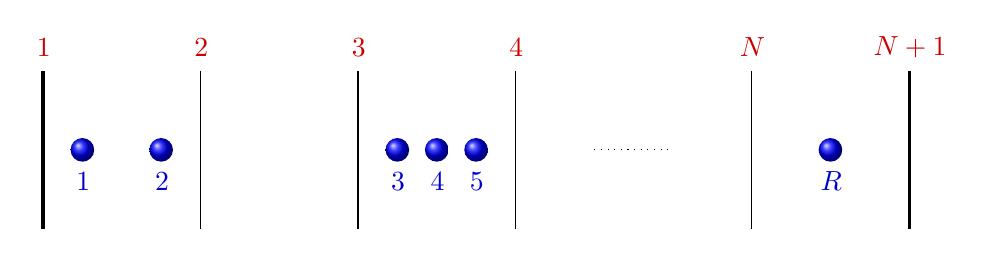
\begin{tikzpicture}
  \draw[very thick] (0.0,0.0) -- (0.0,2.0);
  \draw (2.0,0.0) -- (2.0,2.0);
  \draw (4.0,0.0) -- (4.0,2.0);
  \draw (6.0,0.0) -- (6.0,2.0);
  \draw (9.0,0.0) -- (9.0,2.0);
  \draw[very thick] (11.0,0.0) -- (11.0,2.0);
  
  \draw[dotted] (7.0,1.0) -- (8.0,1.0);
  
  \shade[ball color=blue] (0.5,1.0)  circle (.15cm);
  \shade[ball color=blue] (1.5,1.0)  circle (.15cm);
  \shade[ball color=blue] (4.5,1.0)  circle (.15cm);
  \shade[ball color=blue] (5.0,1.0)  circle (.15cm);
  \shade[ball color=blue] (5.5,1.0)  circle (.15cm);
  \shade[ball color=blue] (10.0,1.0) circle (.15cm);
 
  \draw [red!80!black](0.01,2.3)  node{$1$};
  \draw [red!80!black](2.01,2.3)  node{$2$};
  \draw [red!80!black](4.01,2.3)  node{$3$};
  \draw [red!80!black](6.01,2.3)  node{$4$};
  \draw [red!80!black](9.01,2.3)  node{$N$};
  \draw [red!80!black](11.01,2.3) node{$N+1$};

  \draw [blue!80!black](0.51,0.6)  node{$1$};
  \draw [blue!80!black](1.51,0.6)  node{$2$};
  \draw [blue!80!black](4.51,0.6)  node{$3$};
  \draw [blue!80!black](5.01,0.6)  node{$4$};
  \draw [blue!80!black](5.51,0.6)  node{$5$};
  \draw [blue!80!black](10.01,0.6) node{$R$};
\end{tikzpicture}

  \caption{Conteggio degli stati come permutazione tra $N-1$ linee e $R$ palline. La prima e l'ultima linea, in grassetto, sono fisse e non soggette a permutazione. La prima scatola (cioè il primo oscillatore) contiene $2$ palline (il primo oscillatore è sul secondo livello di energia). La seconda scatola nessuna pallina (il secondo oscillatore è nel {\em ground--state}). La terza scatola contiene $3$ palline, e così via. L'ultima scatola contiene solo una pallina.}
  \label{fig:scapal}
\end{figure}
%%%%%%%%%%%%%%%%%%%%%%%%%%%%%%%%%%%%%%%%%%%%%%%%%%%%%%%%%%%%%%%%%%%%%%%%%

Otteniamo dunque
\be
W = \frac{(N-1+R)!}{(N-1)!R!} \simeq \frac{(N+R)!}{(N)!R!}
\ee
in cui nell'ultimo passaggio abbiamo considerato che $N$ e $R$ sono molto maggiori di $1$. Come nel caso dell'oscillatore singolo ci mettiamo in una situazione semiclassica, ossia valori dell'energia dei singoli oscillatori molto grandi rispetto a $\hbar\omega$. Questo corrisponde a dire che $R \gg N$, e possiamo quindi scrivere
\be
W = \frac{1}{N!}\frac{(R+N)(R+N-1)(R+N-2)\cdots(R+1)R!}{R!} \simeq \frac{R^N}{N!}
\ee
Se ora consideriamo il solito guscio di spessore $\Delta$ intorno all'energia $E$ otteniamo:
\bea
R_+ &=& \left(E+\frac{\Delta}{2}-\frac{N\hbar\omega}{2}\right)\frac{1}{\hbar\omega}\nonumber\\
R_- &=& \left(E-\frac{\Delta}{2}-\frac{N\hbar\omega}{2}\right)\frac{1}{\hbar\omega}
\eea
e otteniamo subito
\bea
\Gamma &=& \frac{1}{N!}(R_+-R_-)\nonumber\\
       &=& \frac{1}{N!}\frac{E^N}{(\hbar\omega)^N}\left[\left(1+\frac{\Delta-N\hbar\omega}{2E}\right)^N -
       \left(1-\frac{\Delta+N\hbar\omega}{2E}\right)^N\right]
\eea
e usando lo sviluppo $(1\pm x)^n\simeq 1\pm nx$ otteniamo subito
\be
\Gamma = \frac{\Delta E^{N-1}}{(N-1)!(\hbar\omega)^N}
\ee
e dal confronto con l'espressione per $\gamma$ troviamo immediatamente
\be
\gamma_0 = h^N
\ee

%%%%%%%%%%%%%%%%%%%%%%%%%%%%%%%%%%%%%%%%%%%%%%%%%%%%%%%%%%%%%%%%%%%%%%%%
\subsection{La regola generale}
%%%%%%%%%%%%%%%%%%%%%%%%%%%%%%%%%%%%%%%%%%%%%%%%%%%%%%%%%%%%%%%%%%%%%%%%

I tre esempi appena visti ci lasciano intuire la regola generale, che è questa: per ottenere il numero di microstati per un sistema classico con $M$ gradi di libertà totali con volume microcanonico $\gamma$ nello spazio delle fasi, occorre dividere $\gamma$ per $h^M$.

Ricordiamo che in ogni caso il vero conteggio del numero dei microstati dovrebbe essere ottenuto con il formalismo quantistico. Il fattore di conversione $h^M$ può essere compreso intuitivamente considerando le relazioni di indeterminazione di Heisenberg: se pensiamo a un sistema unidimensionale con una sola particella è chiaro che a livello quantistico non possiamo determinare contemporaneamente e con posizione arbitraria posizione e momento della particella, ma abbiamo, al meglio
\be
\delta q \delta p \sim \hbar
\ee
Dunque un particolare microstato del sistema occupa, nello spazio delle fasi, un volumetto di ordine $h$. Il risultato si generalizza subito a sistemi con $M$ gradi di libertà.

%%%%%%%%%%%%%%%%%%%%%%%%%%%%%%%%%%%%%%%%%%%%%%%%%%%%%%%%%%%%%%%%%%%%%%%%
\section{Esercizi per il capitolo \ref{cap:elementi}}
%%%%%%%%%%%%%%%%%%%%%%%%%%%%%%%%%%%%%%%%%%%%%%%%%%%%%%%%%%%%%%%%%%%%%%%%

%-----------------------------------------------------------------------
% ESERCIZIO ULTRARELATIVISTICO
%-----------------------------------------------------------------------
\begin{Exercise}[title={Gas ideale ultrarelativistico},label={ex:03-gicur}]
Si consideri un gas ideale composto da $N$ particelle ultrarelativistiche racchiuse in un volume $V$. Sia $E$ l'energia totale del sistema, con $E = \mathrm{costante}$. Si calcoli, col formalismo microcanonico, la relazione che lega la pressione all'energia. Si dimostri inoltre che nel caso ultrarelativistico 
\be
\gamma\equiv C_P/C_V = 4/3\nonumber
\ee
\end{Exercise}

%-----------------------------------------------------------------------
% ESERCIZIO OSCILLATORI DI FERMI
%-----------------------------------------------------------------------
\begin{Exercise}[title={Oscillatori di Fermi},label={ex:03-oscfermi}]
Si consideri un sistema composto da $N$ ``particelle'' non interagenti e distinguibili, ognuna delle quali può stare in due livelli di energia, $\pm\varepsilon$. Sia $E$ l'energia (fissata) del sistema. Si ricavi la temperatura microcanonica d'equilibrio $T$ e si calcoli il numero d'occupazione medio dei due livelli in funzione della temperatura $T$, discutendo i limiti $T\to 0$ e $T\to\infty$.
Si calcoli inoltre l'entropia $S$ come funzione dell'energia $E$, discutendo il comportamento di $S$ per $E > 0$: cosa implica, per la temperatura $T$, che $E$ sia maggiore di zero?
\end{Exercise}

\newpage

%-----------------------------------------------------------------------
% ESERCIZIO OSCILLATORI DI FERMI CON DEGENERAZIONE
%-----------------------------------------------------------------------
\begin{Exercise}[title={Sistema a due livelli con degenerazione},label={ex:03-quasioscfermi}]
Si consideri un sistema di $N$ particelle identiche ma distinguibili e non interagenti. Il sistema ammette due livelli di energia di singola particella: $E_0 = 0$ e $E_1 = \varepsilon > 0$. 
Il livello di energia $E_1$ è $g$-degenere mentre il livello $E_0$ è non degenere. 
Sia $E = n_1\varepsilon$ l'energia totale del sistema ($n_1$ è il numero medio di particelle sul livello di energia $E_1$). 
\begin{enumerate}
  \item Usando il formalismo dell'ensemble microcanonico trovare il numero di occupazione $n_1$ (per le particelle nel livello a energia $E_1$) e $n_0$ (per le particelle nel livello a energia $E_0$) in funzione della temperatura d'equilibrio $T$.
  \item Si consideri il caso in cui $g=2$. Se il sistema ha energia $E=0.75\,N\varepsilon$ ed è posto in contatto termico con una riserva termica a temperatura costante $T= 500\,K$, in che direzione fluisce il calore?
\end{enumerate}
\end{Exercise}

%-----------------------------------------------------------------------
% ESERCIZIO SPIN 1
%-----------------------------------------------------------------------
\begin{Exercise}[title={Particelle di spin 1}, label={ex:03-spin1}]
Si consideri un sistema composto da $N$ particelle non--interagenti e indistinguibili. L'hamiltoniana totale del sistema è
\be
\Ham = -h\sum_{i=1}^N \sigma_i \quad\quad \sigma_i = -1, 0, 1
\ee
dove $h$ una costante con le dimensioni di un'energia. Si può immaginare che le particelle abbiano spin $1$, quindi un certo momento magnetico in direzione $z$, e che $h$ sia il prodotto scalare di un campo magnetico esterno per il momento magnetico delle particelle.

Sia $E$ l'energia, fissata, del sistema. Chiamando $N_\sigma$ il numero d'occupazione del livello $\sigma$, con $\sigma = -1, 0, 1$, si calcoli, utilizzando il formalismo microcanonico, il rapporto $N_{-1}/N_{1}$ in funzione della temperatura $T$ d'equilibrio. Si calcoli inoltre $A(N,T)$, l'energia libera di von Helmholtz.

Si confronti il risultato con quello ottenuto utilizzando il formalismo canonico (vedi Capitolo \ref{cap:canonico}).
\end{Exercise}

%%%%%%%%%%%%%%%%%%%%%%%%%%%%%%%%%%%%%%%%%%%%%%%%%%%%%%%%%%%%%%%%%%%%%%

\vskip 0.75cm
\begin{flushright}
{\em Ultimo aggiornamento del capitolo: 21.04.2017}
\end{flushright}
